\section{Experimental Evaluation}

\JZ{Having results using a recursive variant of SLEM would be interesting. Classificaiton results using $K$-NN or Nearest Class Mean (NCM) classifiers (or SVMs) would be interesting too, as done in the E-SVM paper.}

\subsection{Datasets and evaluation protocol} \label{eval:protocol}
Our default dataset in this paper will be INRIA \emph{Holidays} dataset \cite{holidays}. This dataset consists of 1491 images divided in 500 groups of matching images. For the remaining of this report, if the dataset of an experiment is not mentioned, the experiment is performed on \emph{Holidays}.
We also perform in the \emph{Oxford} dataset \cite{oxford}, which consists of 5062 images separated in 55 groups of matching images.

Each group of these datasets contains one query image. For each query image we rank all the other images in the dataset based on the similarity between them and the query image, in decreasing order. The average precision of a group is calculated by the ranking of the images of the group for the similarity with the corresponding query image. The final mean average precision (mAP) for a dataset is the mean of the average precision over all its groups.
As negative sample of images, we use a small set of images from Flickr100K \cite{oxford}.

At evaluation time, for a dataset that consists of $p$ images and $q$ query images, we calculate its $p\times q$ \emph{similarity matrix} $S$, where each of its $q$ columns is the matching scores of the query image with all the $p$ images.
\subsection{Base Encoding of Images}
We use three base features as the representation in $\RR^d$ of our images. Firstly, we use VLAD representation, as used in \cite{ZePe15}. 
CNN features are non-negative and can be used both as $\mathbb{L}^1$ or $\mathbb{L}^2$ normalized features. The third features are spatial pyramids of SIFT descriptors, as used in \cite{spk}. These are non-negative $\mathbb{L}^1$ normalized features. \emph{\color{red} Details of these features construction are not relevant right now.}
\subsection{Implementation details}
\emph{\color{red} Not relevant right now.  To be written.}
$8192$ dimensional VLAD features.

E-SVM: $0.6$ second to solve one single exemplar.

SLEM: $30$ seconds to solve a $8192\times 8192$ linear system for all exemplars of the dataset.

Kernelized SLEM: at most $0.3$ seconds (for RBF kernel) for each iteration of (\ref{icd:algo}) algorithm plus at most $30$ seconds to solve a $r'\times r'$ system.

\begin{table*}[t]
\begin{center}
\begin{tabular}{|c|c|c|c|c|c|}
\hline
Method, features & VLAD-64 \cite{VLAD}& CNN \cite{jia2014caffe} & SP-SIFT \cite{spk} & SPoC CNN \cite{babenko15} &  SP-CNN \cite{SPPCNN} \\
\hline\hline
Baseline            & 72.7 & 68.2 & 37.4 & 73.1 & 64.7\\
%Whitening           & -    & -    & -    & -    & -\\
LDA                 & 69.4 & 69.2 & -    & 77.5 & -\\
E-SVM               & 77.5 & 71.3 & 40.1 & 79.8 & 64.7 \\
Linear SLEM         & 77.9 & 72.1 & 38.2 & 78.3 & 68 \\
Gaussian SLEM       & 78.1 & 72.9 & 39.7 & 79.8 & 68.6 \\
Intersection SLEM   & -    & 70.2 & 66.9 & -    & 70.2 \\
\hline
\end{tabular}
\end{center}
\caption{Mean average precision results for INRIA Holidays dataset, expressed as percentages. The - means the tests can not be performed or was not performed yet.}
\end{table*}


\begin{table*}[t]
\begin{center}
\begin{tabular}{|c|c|c|c|c|c|}
\hline
Method, features & VLAD-64 \cite{VLAD}& CNN \cite{jia2014caffe} & SP-SIFT \cite{spk} & SPoC CNN \cite{babenko15} &  SP-CNN \cite{SPPCNN} \\
\hline\hline
Baseline            & 46.3 & 40.6 & - & 54.4 & 44 \\
%Whitening           & 07   & 20.2 & - & -    & -\\
LDA                 & 50.9 & 45   & - & 63.7 & 37.4\\
E-SVM               & 57.5 & 44.6 & - & 62.1 & - \\
Linear SLEM         & 57.5 & 45.5 & - & 64.1 & 45 \\
Gaussian SLEM       & 59   & 46.1 & - & 64.9 & 45 (no cv) \\
Intersection SLEM   & -    & 42.2 & - & -    & - \\
\hline
\end{tabular}
\end{center}
\caption{Mean average precision results for Oxford 5k buildings dataset, expressed as percentages. The - means the tests can not be performed or was not performed yet.}
\end{table*}


\subsection{Low-rank decomposition evaluation}

\begin{figure}[!h]
\centering
\begin{subfigure}[b]{0.48\textwidth}
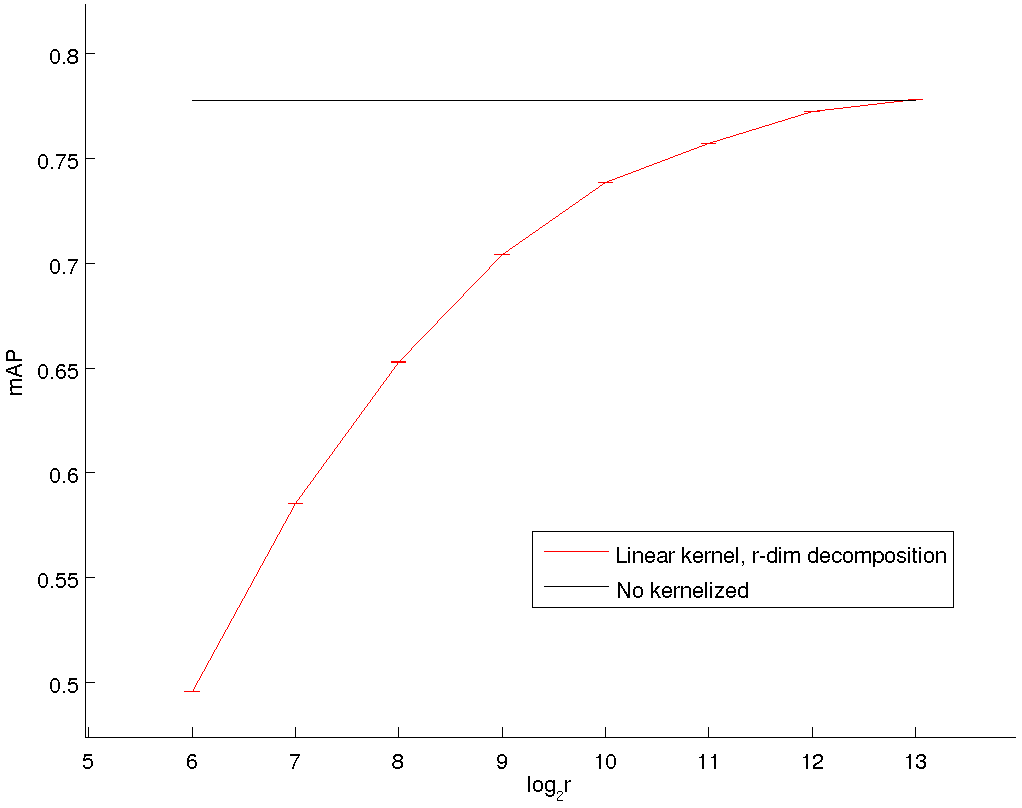
\includegraphics[width=\textwidth]{None_vs_linear.png}
\end{subfigure}
\begin{subfigure}[b]{0.48\textwidth}
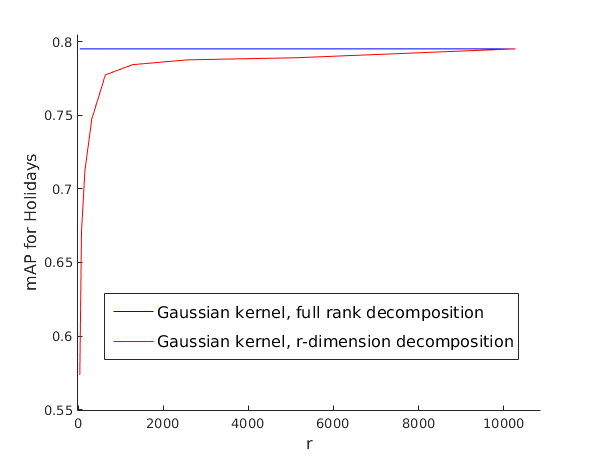
\includegraphics[width=\textwidth]{rbf_decomposition_nolog.png}
\end{subfigure}
\caption{At the left, comparison between no kernel results and linear kernel results. In black, mAP of non kernelized SLEM. In red, mAP for different low-rank decompositions of linear kernel matrix. In this experiment, $r=2^{13}$ and we set $\log_2 r'$ in $\{6, 7,...,13\}$. At the right, comparision between the Gaussian kernel results and its low-rank decomposition results. In blue, mAP of the full-rank Gaussian SLEM. In red, mAP for different low-rank decomposition of Gaussian SLEM. In this experiment, $r=10281$.}
\label{no.ker.vs.linear2}
\end{figure}

\subsection{Time Scalability}
\begin{figure}[!h]
\centering
\begin{subfigure}[b]{0.48\textwidth}
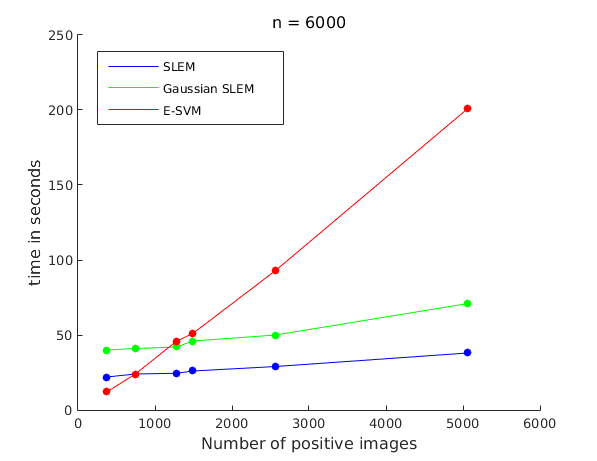
\includegraphics[width=\textwidth]{speed_n_6K.png}
\end{subfigure}
\begin{subfigure}[b]{0.48\textwidth}
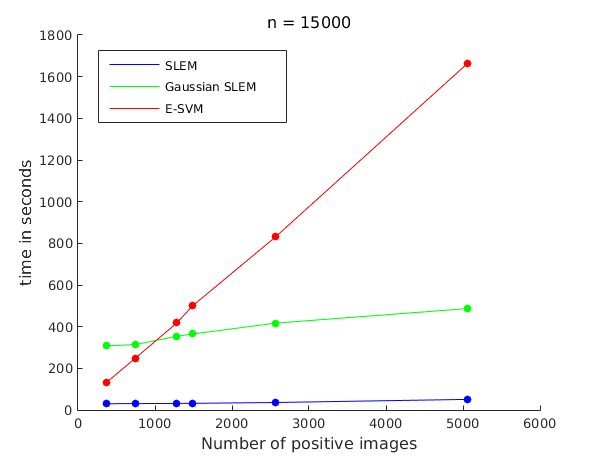
\includegraphics[width=\textwidth]{speed_n_15K.png}
\end{subfigure}
\caption{Comparison between time calculation of similarity matrix $S$, as defined in \ref{eval:protocol}, for different methods. \JZ{Not too sure what this is... Does it include the feature computation time for all positives/negatives? If so, then why call it \emph{time calculation of similarity matrix}? Or is it just the score computation, in which case, shouldn't the complexity be the same for SLEM and E-SVM?}}
\label{time:scalar}
\end{figure}

%\caption{Comparison between no kernel results and linear kernel results. In black, mAP of non kernelized SLEM. In red, mAP for different low-rank decompositions of linear kernel matrix. In this experiment, $r=2^{13}$ and we set $\log_2 r'$ in $\{6, 7,...,13\}$. }

%\caption{Comparison between no kernel results and linear kernel results. In black, mAP of non kernelized SLEM. In red, mAP for different low-rank decompositions of linear kernel matrix. In this experiment, $r=2^{13}$ and we set $\log_2 r'$ in $\{6, 7,...,13\}$. }


%%% Local Variables:
%%% TeX-master: "main_eccv"
%%% End: